\documentclass[11pt]{article}
\usepackage{report}
\usepackage{times}
\usepackage{url}
\usepackage{latexsym}
\usepackage{tikz}
\usepackage{pgfplots}
\usepackage{amsmath}
\usepackage{multirow}% http://ctan.org/pkg/multirow

\DeclareMathOperator*{\argmax}{argmax}


\title{A tweet can contain 140 characters but a picture is worth 1000
  words\thanks{~~\emph{Christopher Jenkins, 2017}}}

\author{Simon Tannert~~~ \\
  {\tt tannersn@ims.uni-stuttgart.de~~~} \\\And
  ~~~Touhidul Alam \\
  {\tt ~~~alamtl@ims.uni-stuttgart.de} \\}

\date{}

\begin{document}
\maketitle
\begin{abstract}
  This report contains the analysis of emotion prediction based on tweet corpus. The objective of the experiment is to predict emotion based on text and image associated with it. We use Naive Bayes and perceptron classifier to predict emotion from the tweet text. Also with the perceptron, we experiment tweet image and the text combinination. Furthermore, we use a convolutional neural network model that predicts based on both text and image of tweet and later we discuss the comparison between different of these models.
\end{abstract}

\section{Introduction}

On social media, everyday people shares a lot of content which depicts their opinion or sentiment of matters in form of text or media. By analyzing the contents of these texts or media from social media e.g: Facebook, Twitter, Instagram etc., we can predict some insight about the reaction of people towards some specific topic or products. Companies can use these data analysis to assess the quality of their services, public figures and their popularities.

Other than texts, the role of pictures in conveying emotional message and opinion is recognized as important. In social media, many now uses image as an expression to one's opinion. So as an additional resources in this experiment we also focuses on image data as a source of emotion prediction. On our given context around 30\% of data contains image. We evaluate primary image features (e.g., brightness, color) that are more visually related to the emotional content of an image and allow a better image classification, that can be used to predict the emotion conveyed by images. 

We experiment different approach for text, image and combination of both data in our implemented classifier. First we compare a simple naive bayes and Perceptron classifier based on text features. Later we augmented our perceptron to classify image data in combined with text result features. Further we implemented a Convolutional Neural Network that combined with both text and image input data.

\section{Methods}
\label{sec:methods}

We explore two different approaches to emotion detection.
In the first approach, we consider only the text in the body of the tweets.
In our second approach, we look at tweets that come with a picture and use it as
an additional information source.

We implemented several classifiers for the two approaches which we will present
in the following.

\subsection{Text-based Classification}

For the text-based approach, we implemented three classifiers, Naive Bayes, a
multi-class Perceptron and a simple neural network which learns word embeddings
to derive a document representation.

\subsubsection{Naive Bayes}
\label{sssec:naive_bayes}

Naive Bayes estimates the joint probability of a datum in the corpus represented
by features and its assigned class.

We can train such a model with a corpus from which we take both class frequency
and the relative frequency of features we extract from every document that
belongs to a certain class.
We can then estimate each class's prior probability $p(C_k)$ and the conditional
probability $p(C_k|x)$ for every class and feature. 
Once we trained such a model, we can get a class prediction for a feature vector
x with the following formula

\begin{equation}
  y = \underset{k\in\{1,\ldots,K\}}{\argmax}p(C_k)\prod_{i=1}^{n}p(\textrm{x}_i|C_k)
\end{equation}

This approach cannot deal with features that have not been seen during training,
because their conditional probability is zero, which would make the entire product
zero.
To tackle this we use Laplace smoothing for all words that appear only in the
test corpus to give them a small non-zero probability

\begin{equation}
\theta_i = \frac{x_i + \alpha}{ N + \alpha d} \;\; (i = 1,2...d)
\end{equation}

The hyperparameter $\alpha>0$ controls how much probability mass we shift over to
unseen features and has to be determined empirically.

A straightforward way to extract features from documents is to take the surface
form of each word as feature.
This is called bag-of-words because it ignores the position the words appear in
in the document but it works reasonably well.

On top of that we also use the concatenation of pairs of neighboring words as
features.

\subsubsection{Perceptron}
\label{sssec:perceptron}

A perceptron is a linear classifier which, in its base form, estimates a
hyperplane between vectors from either of two classs we want to discriminate.
The perceptron comprises a weight vector, which stores weights for every feature
encountered during training. To get a prediction for a vector x, we use the
following algorithm.

\begin{equation}
  f(x) = \begin{cases}
    1, & \text{if}\ \sum_{k=1}^K w_k \cdot x_k + b > 0\\
    0, & \text{else}
         \end{cases}
\end{equation}

where $w_k$ are the weights from the weight vector corresponding to the features
$f_k$ in the input vector.

To train the perceptron, we have to update the weights $w_k$. To do so, we first
get a prediction from the perceptron with above formula. If the prediction was
wrong, we adjust the hyperplane towards the correct prediction with the
following algorithm.

\begin{equation}
  w = w + (f(x) - y) \cdot x
\end{equation}

where $f(x)$ is the predicted class and y the actual class.

For our task, we use a modification of the binary perceptron that allows
multi-class classification.
We achieve this by using one weight vector per class we encounter in the
training data. For prediction we then use

\begin{equation}
  \argmax_j \sum_{k=1}^K w_{j,k} \cdot x_{j,k}
\end{equation}

which returns the class whose weights maximise the equation for the current
vector.
If predicted and actual class differ, we penalize the predicted class by
adding $-\text{x}$ to its weights and boost the actual class by adding x to its weights.

We use a technique called averaging to mitigate the effect of the order of the
training on the instances on the weights.
In an unaveraged Perceptron, later training instances have a larger effect on
the weight vector.
Averaging is done by keeping track of when an update to a particular feature
occured and subsequent rescaling of the weights after each epoch.

Like in the Naive Bayes classifier, we use bag-of-words features and
features that model pairs of neighboring words.
These features are binary, which means that the feature corresponding to a word
is 1 when it appears in a particular document and 0 else.

In addition to these we also use the following word based features\\

\begin{tabular}{|r|l|}
  \hline
  feature & description\\\hline\hline
  is\_alpha & contains only alpha characters\\
  is\_digit & contains only numeric characters\\
  is\_lower & is in lower case\\
  is\_upper & is in upper case\\
  is\_title & is in title case\\
  first2 & the first two characters\\
  last2 & the last two characters\\
  first3 & the first three characters\\
  last3 & the last three characters\\
  first4 & the first four characters\\
  last4 & the last four characters\\\hline
\end{tabular}\\~\\

An additional bias feature which is 1 for all training instances allows the
Perceptron algorithm to shift the hyperplane along that dimension if necessary.

\subsubsection{Min-Max Neural Network}
\label{sssec:mmnn}

A third approach we implemented was a simple neural network which implements the
idea introduced in \cite{de2016representation}.

The network consists of an embedding layer, which learns word embeddings.
For each tweet, two vectors are constructed by taking all the maximum values
of each dimension of the embedding vectors that comprise the document.
The same is done for the minima and the resulting vectors are concatenated to
form a representation for the document.

This document representation is then fed into a softmax layer to predict an
emotion class.

\subsection{Picture-based Classification}

Many tweets come with pictures, which we want to use as an additional source of
information for emotion detection.
If we model emotion detection as a generative process, we imagine that the
author of a particular tweet wants to convey a certain emotion and we can find
clues of it in the content.
In that sense, we assume that the picture that accompanies a tweet was selected
with the intention to convey the same emotion but contains information that is
not yet in the body of the tweet.

Previous work in this area \cite{Klinger2017} tried to use the pictures by
extracting text from them using optical character recognition.
They then proceeded to train a model on bag-of-words features extracted from both
body and the text from the picture.

Our approach is to extract features from the pictures directly. In the following
we present two methods we investigated.

\subsubsection{Perceptron}

First we wanted to test if we can extract meaningful features via handcrafted
templates that consider latent picture features such as brightness, hue and
saturation.

To do so, we use the histograms of brightness, hue and saturation and construct
real-valued features out of every rank.
As this would result in a lot of features, we decided to reduce the picture
resolution before we get the histograms to make it computationally feasible.
As a second optimization step we reduce the dimensionality of the resulting
histograms by binning the ranks and interpolating linearly between bins.

We reuse the Perceptron we introduced in Section
\ref{sssec:perceptron} to train a model with the picture features.

We expect the pictures to have three channels, red, green and blue, before we
extract features.
We convert grayscale pictures to RGB by repeating the channel three times.
If a grayscale or RGB picture has an alpha channel, we simply drop the alpha
channel.

Figure \ref{fig:hsv_features} shows the process of reducing the picture resolution
and splitting it into brightness, hue and saturation.

\begin{figure*}[ht]
\begin{center}
        \begin{tikzpicture}
          \node(a){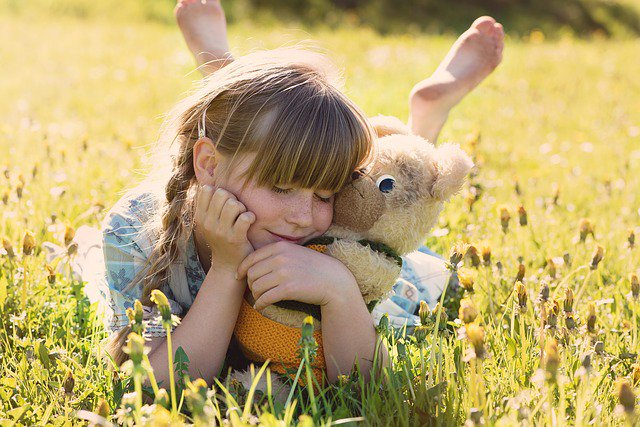
\includegraphics[scale=.15]{../res/804855952797270016.jpg}};
          \node(b)[right of=a,xshift=80pt,yshift=-10pt]{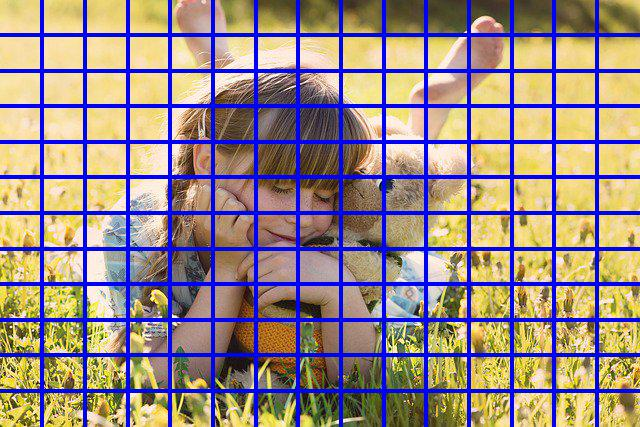
\includegraphics[scale=.15]{../res/804855952797270016_grid.jpg}};
          \node(c)[right of=b,xshift=80pt,yshift=-10pt]{
\includegraphics[scale=.15]{../res/804855952797270016_med.jpg}};
          \node(d)[below of=c,xshift=-105pt,yshift=-50pt]{
\includegraphics[scale=.15]{../res/804855952797270016_lum.jpg}};
          \node(e)[below of=c,xshift=0pt,yshift=-50pt]{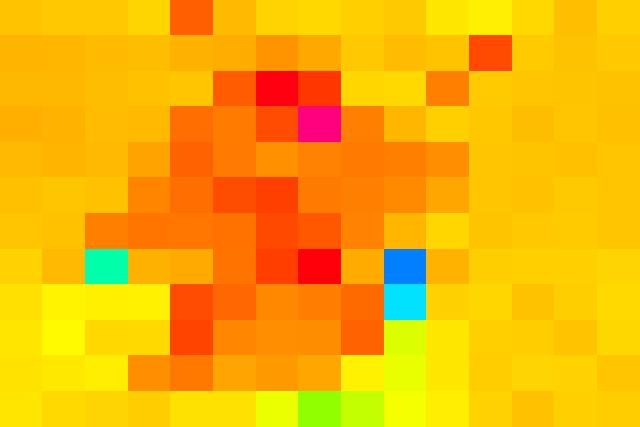
\includegraphics[scale=.15]{../res/804855952797270016_hue.jpg}};
          \node(f)[below of=c,xshift=105pt,yshift=-50pt]{
\includegraphics[scale=.15]{../res/804855952797270016_sat.jpg}};

          \node(hd)[below of=d,yshift=-15pt] {Brightness};
          \node(he)[below of=e,yshift=-15pt] {Hue};
          \node(hf)[below of=f,yshift=-15pt] {Saturation};

          \draw[->](a) -- (b);
          \draw[->](b) -- (c);
          \draw(c) -- (d);
          \draw(c) -- (e);
          \draw(c) -- (f);
        \end{tikzpicture}\vspace*{-0pt}
        \caption{Picture Feature Extraction}
        \label{fig:hsv_features}
\end{center}
\end{figure*}

\subsubsection{Convolutional Neural Network}
\label{sssec:cnn}

In our second approach, we use a convolutional neural network (CNN) to classify
emotions.

Their main advantage which make them appealing for the task at hand is that they
do not require features to be designed before training.
Instead, so-called filters process the picture and automatically learn features
that are suitable to discriminate the emotion classes.

Another advantage is that CNNs can be implemented efficiently and thus can be
trained in a relatively short time.

We chose a shallow network structure, consisting of three filter layers, which
each feed into separate a max-pooling layer. The max-pooling layers are
concatenated and then a softmax layer is used to get predictions for the target
emotion classes.

\subsection{Combined Classification}

At this point we have both text- and picture-based predictions from two
different models.
In this section we describe how we combined them into models that use both text and picture information during training.

\subsubsection{Perceptron}

The naive approach we explored first is to just use both the text and picture
features to train the same Perceptron.
Initial experiments showed that this this does not work and we did not explore
it any further.

We suspect that this is due to how different the features are: The text features
are sparse and take only binary values while the picture features are dense in
comparison and real-valued.

Our second approach was to use two Perceptron classifiers.
One of them is trained on the text features first and the other one is trained
on the picture features and the ranked output of the first Perceptron.

To facilitate this, we normalize the picture features to values between 0 and 1
by dividing them by the number of pixels in the picture.

To turn the ranked output of the first Perceptron into features, we take the raw
output which can take on values between $-\infty$ and $+\infty$ and apply
softmax to them to also get them in the range between 0 and 1.

\subsubsection{Min-Max and Convolutional Neural Network}

The two Neural Networks described in Section \ref{sssec:mmnn} and Section
\ref{sssec:cnn} can be combined into a single model easily.

The softmax layer at the end of each network was replaced with a fully connected
dense layer of the same size and the concatenated output of both dense layers
fed into the softmax layer for prediction.

\section{Experiments}

In this Section we introduce the corpus we worked with and the experiments we
conducted with the models introduced in Section \ref{sec:methods}.

\subsection{Corpus}
For our experiments, we were provided with a 1.63 million tweet corpus.
It comprises tweets in several languages with the three most popular being English
(71.4\%), Spanish (8.9\%) and German (3.2\%).
The corpus is split into training and test set in a 3:1 ratio.
31\% of the tweets in the training set and 25\% of the tweets in the test set
come with a picture.
The distribution of emotion classes can be seen in Figure \ref{fig:corpus}

\begin{figure}
\pgfplotsset{every tick label/.append style={font=\tiny}}
\begin{tikzpicture}[trim axis left]
\begin{axis}[
  height=150pt,
  width=255pt,
  ytick={0,10,20,30,40,50},
  yticklabels={0\%,10\%,20\%,30\%,40\%,50\%},
  xticklabels={,happy,love,sad,anger,fear,surprise,disgust,trust}]
\addplot+[ybar] plot coordinates
  {(0,48.98) (1,18.57) (2,14.88) (3,7.47) (4,6.88) (5,2.77) (6,2.28) (7,2.16)};
\end{axis}
\end{tikzpicture}
\caption{Distribution of emotion classes}
\label{fig:corpus}
\end{figure}
\begin{center} \end{center}

We use the corpus as is, meaning that we do not filter out languages or
preprocess the text in the body.
We explored different ways of preprocessing, like stop word lists, removal of
newlines, removal of the hash sign from hashtags and replacing usernames with
placeholders, but they all had a detrimental effect on our models.

\subsection{Experimental Settings}
\label{ssec:exsettings}

In this Section we describe how we chose the hyperparameters for our experiments.
All our models are trained on the full training data and tested on the full
training set.
Note that these sets are smaller for the approaches using picture data.

For the approaches that use pictures as input, we do the picture scaling in
parallel with imagemagick \footnote{https://imagemagick.org} before we load them
into memory.

Both text and picture feature extraction are also done in parallel and then
cached for subsequent epochs to speed up training.

\subsubsection{Text-based Classification}

\subsubsection*{Naive Bayes}
We experimentally determined that setting $\alpha=0.06$ gives us the best
results in the Naive Bayes classifier.

\subsubsection*{Min-Max Neural Network}
In the Min-Max Neural Network, we use word embeddings of length 30 and thus
document vectors of length 60.

\subsubsection{Picture-based Classification}
\subsubsection*{Perceptron}
When we extract the picture feature vectors for Perceptron training, we first
scale the pictures to 12*12 which gives us a total of 144 pixels.
The brightness and saturation histograms are binned from 256 ranks to 8 feature
bins, the raw hue output is binned from 360 ranks to 9.

\subsubsection*{Convolutional Neural Network}
Before the pictures are fed into the network they are resized to 128*128 so they
can all be loaded into memory and to speed up training.
We use 20 filters of size 1*1, 16 filters of size 3*3 and 12 filters of size
5*5.
Each filter layer feeds into a 2*2 max-pooling layer.

\subsubsection{Combined classification}

\subsection{Results}
\label{ssec:results}

We have observed variations of score in different approach. From the Table 1 and Table 2, For the Naive Bayes classifier, we observe average F1-score 41\% on evaluation set while ``happy'' label scores the highest  71\% and ``trust'' lowest score .78\%. On perceptron text classification after 13 epochs, we observe an average 57\% F1-score, which is siginifantly higher than simple Naive Bayes approach. while ``happy'' and ``sad'' labels are dominant respectively 78\% and 71\% with f-score.

In perceptron with image classifier,
 
\begin{table*}
\begin{center}
  \caption{Result}
  
  \begin{tabular}{|c||l|l|l|l|l|l|l|}
  \hline
  \multirow{2}{*}{Score} 
      & \multicolumn{3}{c|}{Text-based } 
          & \multicolumn{2}{|c|}{Picture-based }
          &          \multicolumn{2}{|c|}{Combined} \\             \cline{2-8}
  & Naive Bayes & Perceptron & Min-Max NN & Perceptron & CNN & Perceptron & Min-Max CNN   \\  \hline
  $Macro$ & 1 & 2 & 3 & 1 & 2 & 3 & 5 \\      \hline
  $Accuracy$ & 1 & 2 & 3 & 1 & 2 & 3 & 3 \\      \hline
\end{tabular}

\end{center}
\end{table*}


\subsection{Error Analysis}
\label{ssec:erroranalysis}



\section{Summary and Conclusions}


\section{Future Work}
\label{sec:length}


% include your own bib file like this:
\bibliographystyle{acl}
\bibliography{report}

\end{document}
